%%This is a very basic article template.
%%There is just one section and two subsections.
\documentclass[a4paper, ngerman]{scrartcl}

\usepackage[T1]{fontenc}
\usepackage[utf8]{inputenc}
\usepackage[ngerman]{babel}
\usepackage{lmodern}
\usepackage{amsmath}
\usepackage{amsfonts}
\usepackage{hyperref}
\usepackage{graphicx}
\usepackage{paralist}
\usepackage[none]{hyphenat}
\usepackage{wrapfig}
\usepackage{subfig}
\usepackage{subfloat}

\def\sectionautorefname{Abschnitt}
\def\figureautorefname{Abbildung}

\sloppy



\hypersetup{
pdfborder = {0 0 0},
urlbordercolor = {0 0 0},
colorlinks = true,
linkcolor = black,
citecolor = black,
filecolor = black,
urlcolor  = black
}
\addtolength{\oddsidemargin}{-.875in}
	\addtolength{\evensidemargin}{-.875in}
	\addtolength{\textwidth}{1.75in}

	\addtolength{\topmargin}{-.875in}
	\addtolength{\textheight}{1.75in}

\captionsetup[figure]{skip=5pt}

\title{Software-Challenge 2014 - Sixpack}
\subtitle{Spielregeln}



%% Variablen
\newcommand{\SpielFelderAnzahl}{\emph{256}}
\newcommand{\KartenAnzahl}{\emph{KartenAnzahl}}
\newcommand{\PiratenAnzahl}{\emph{6}}
\newcommand{\EmptyPlainPage}{\newpage\thispagestyle{plain}\ \newpage}
\newcommand{\RundenAnzahl}{\emph{15}}

\begin{document}

\section*{Sixpack Kurzanleitung} Zu Spielbeginn erhält jeder Spieler 6
Steine, die unterhalb des Spielbretts offen liegen, so dass der Gegner diese sehen kann.
Im Vorrat befinden sich dann noch 96 Steine, von denen 12 aufgedeckt sind. Der
rote Spieler beginnt.\\
 Jeder Spieler hat in seinem Zug zwei verschiedene Möglichkeiten. Entweder er
 legt einen oder mehrere Spielsteine auf dem Spielbrett aus, oder er tauscht
 zwischen 1 und 6 seiner Spielsteine gegen neue ein. Im ersten Zug müssen
 mindestens 2 Spielsteine ausgelegt werden. Ist dies nicht möglich, so muss der
 Spieler Steine tauschen.
Beim Anlegen gelten folgende Regeln:
\begin{itemize}
\item Eine Reihe besteht entweder aus Spielsteinen, welche die gleiche Farbe oder die gleiche Form besitzen.
\item In einer Reihe von gleichen Formen darf jede Farbe höchstens einmal vorkommen.
\item In einer Reihe von gleichen Farben darf jede Form höchstens einmal vorkommen.
\item Ein Spielstein, der ausgelegt werden soll, muss immer an schon vorhandene Spielsteine angelegt werden. Ausnahme ist hier der als erstes ausgelegte Spielstein einer Partie.
\item Werden mehrere Steine in einem Zug ausgelegt, müssen diese sich in derselben Reihe befinden. Am Ende eines Zuges muss für alle auf dem Spielbrett unmittelbar horizontal oder vertikal nebeneinander liegenden Steine gelten, dass diese ausschließlich die zuvor beschriebenen Reihen bilden.
\end{itemize}
\begin{minipage}[c]{0.4\textwidth}
	\centering
	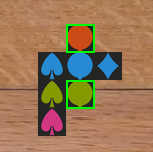
\includegraphics[width=0.5 \textwidth]{images/anlegen04}
	\captionof{figure}{Anlegen von 2 Spielsteinen}
\end{minipage}
\begin{minipage}[c]{0.4\textwidth}
	\centering
	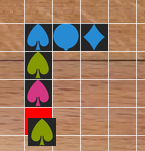
\includegraphics[width=0.5 \textwidth]{images/anlegen02}
	\captionof{figure}{Ungültige Position. Die Reihe hat schon ein Pik derselben Farbe.}
\end{minipage}

Nach dem Anlegen der Spielsteine werden die Steine des Spielers wieder auf 6
aufgefüllt. Die Steine, die dieser erhält, können in der Reihe unterhalb des
Beutels eingesehen werden. Der Spielstein, welcher sich ganz unten befindet, ist der erste, den der Spieler erhält.\\

Ist ein Spieler mit seinen Steinen unzufrieden, kann er zwischen 1 und 6
Spielsteine gegen neue aus dem Vorrat tauschen. Kann ein Spieler keine
Spielsteine anlegen, dann muss er Spielsteine tauschen. Nach dem Tausch ist der
Zug des Spielers beendet.
\newpage
	
 \subsection*{Punkteverteilung}
% \begin{wrapfigure}[10]{R}{0.4\textwidth}
% 	\centering	
% 		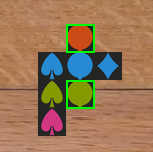
\includegraphics[scale = 0.7]{images/anlegen04}
% 		\caption{Für das Anlegen erhält der Spieler 5 Punkte.}
% 		\label{fig:Punkte1}	
% \end{wrapfigure}
Beim Anlegen von Spielsteinen erhält man einen Punkt für jeden Stein, der sich in einer erweiterten Reihe befindet. Ein Stein wird doppelt gezählt, wenn er Teil von zwei Reihen ist (siehe \autoref{fig:Punkte1}).\\
Wenn man es schafft, eine Reihe von 6 Steinen zu erzeugen, bildet man ein \textbf{Sixpack}, für den es einen Bonus von 6 Punkten gibt (siehe \autoref{fig:PunkteSixpack}).\\
Das Tauschen von Spielsteinen bringt 2 Punkte, unabhängig davon, wie viele
Steine getauscht werden.
\vspace{15pt}

\begin{minipage}[c]{0.4\textwidth}
	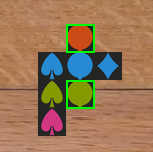
\includegraphics[width=0.5 \textwidth]{images/anlegen04}
	\captionof{figure}{Für das Anlegen erhält der Spieler 5 Punkte.}
	\label{fig:Punkte1}
\end{minipage}
\hspace{0.1\textwidth}
\begin{minipage}[c]{0.4\textwidth}
	\centering	
	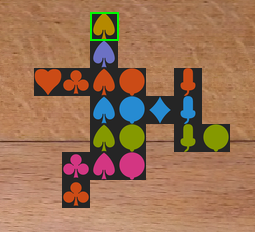
\includegraphics[width=0.5 \textwidth]{images/sixpack_legen}
	\captionof{figure}{Das Anlegen des grün umrandeten Steines ergibt ein
	\emph{Sixpack}. (12 Punkte)}
	\label{fig:PunkteSixpack}
\end{minipage}

% \begin{figure}[h]
% \centering
% 	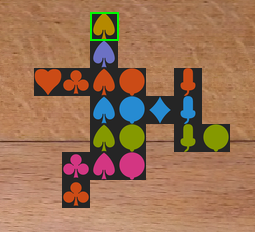
\includegraphics[scale = 0.6]{images/sixpack_legen}
% 		\caption{Das Anlegen des grün umrandeten Steines ergibt ein \emph{Sixpack}. (12 Punkte)}
% 		\label{fig:PunkteSixpack}	
% \end{figure}
	
\end{document}
